\section*{Boosting Signal Strength: The Power of High Reactance!}
\begin{tcolorbox}[colback=gray!10, colframe=black, title=E9D04]
Why should antenna loading coils have a high ratio of reactance to resistance?
\begin{enumerate}
    \item A: To swamp out harmonics
    \item B: To lower the radiation angle
    \item \textbf{C: To maximize efficiency}
    \item D: To minimize the Q
\end{enumerate} \end{tcolorbox}

\subsubsection{Concepts Related to Antenna Loading Coils}
Antenna loading coils are crucial components in radio communication systems, primarily utilized to enhance the performance of antennas by adjusting their impedance characteristics. When designing loading coils, the ratio of reactance (X) to resistance (R), often expressed as \( \frac{X}{R} \), plays a significant role in determining the efficiency of the antenna system.

\subsubsection{Why a High Ratio is Preferred?}
1. \textbf{Maximizing Efficiency:}: A high ratio of reactance to resistance is sought because it ensures that most of the power supplied to the antenna is radiated as electromagnetic waves rather than being dissipated as heat within the coil. High reactance relative to resistance means that the antenna can operate closer to its resonance frequency, minimizing energy loss.

2. \textbf{Impedance Matching:}: Higher reactance values can help in better matching the antenna impedance to that of the transmitter, facilitating efficient power transfer. This is essential in maximizing the overall performance of the antenna system.

3. \textbf{Quality Factor (Q):}: The quality factor (Q) of a circuit is defined as the ratio of its reactance to its resistance. A high Q indicates a narrow bandwidth and better resonance, which means the antenna will be more selective to its desired frequency, improving its performance.

\subsubsection{Mathematical Implication}
If we let \( R \) be the resistance and \( X \) be the reactance of the loading coil, we can define the efficiency \( \eta \) of the loading coil as:
\[
\eta = \frac{P_{radiated}}{P_{input}} = \frac{X^2}{X^2 + R^2}
\]
From this equation, it is evident that increasing \( X \) (while keeping \( R \) constant) leads to an increase in the efficiency \( \eta \), supporting the choice (C) to maximize efficiency.

\subsubsection{Diagrams and Visualization}
To illustrate, consider the following diagram showing the relationship of reactance and resistance in an antenna loading coil:

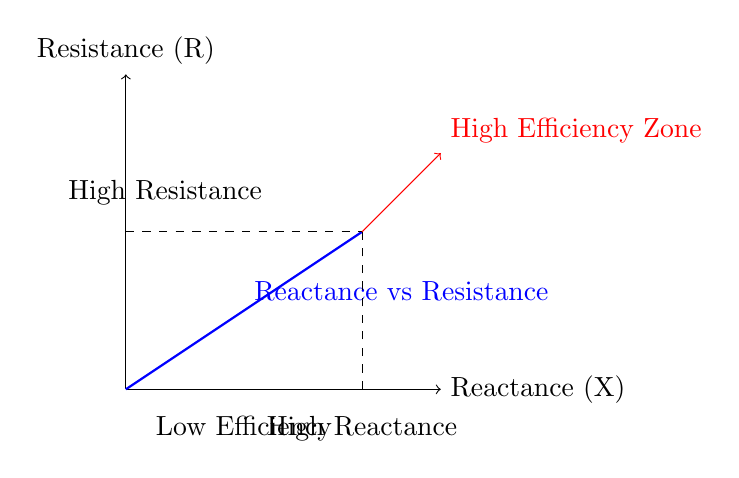
\begin{tikzpicture}
    \draw[->] (0,0) -- (4,0) node[right] {Reactance (X)};
    \draw[->] (0,0) -- (0,4) node[above] {Resistance (R)};
    
    \draw[blue,thick] (0,0) -- (3,2) node[pos=0.5, above right] {Reactance vs Resistance};
    \draw[dashed] (0,2) -- (3,2);
    \draw[dashed] (3,0) -- (3,2);
    
    \node at (1.5, -0.5) {Low Efficiency};
    \node at (3, -0.5) {High Reactance};
    \node at (0.5, 2.5) {High Resistance};
    
    \draw[->, red] (3,2) -- (4,3) node[above right] {High Efficiency Zone};
\end{tikzpicture}
